
\documentclass[12pt,letterpaper]{article}

\usepackage[english]{babel}
\usepackage[utf8]{inputenc}
\usepackage[T1]{fontenc}
\usepackage{fullpage}
\usepackage{cancel}
\usepackage{booktabs}
\usepackage[top=2cm, bottom=4.5cm, left=2.5cm, right=2.5cm]{geometry}
\usepackage{amsmath,amsthm,amsfonts,amssymb,amscd}
\usepackage{lastpage}
\usepackage{enumerate}
\usepackage{fancyhdr}
\usepackage{mathrsfs}
\usepackage{xcolor}
\usepackage{graphicx}
\usepackage{listings}
\usepackage{hyperref}
\usepackage{tikz}
\usepackage{tikz-cd}
\usepackage{pgfplots}
\usepackage{caption}
\usepackage{subcaption}
\usepackage[
backend=bibtex,
sorting=ynt
]{biblatex}
\addbibresource{refs.bib}

\newtheorem{defi}{Definition}
\newtheorem{teo}{Theorem}
\newtheorem{prop}{Proposition}
\hypersetup{%
	colorlinks=true,
	linkcolor=blue,
	linkbordercolor={0 0 1}
}

\setlength{\parindent}{0.0in}
\setlength{\parskip}{0.05in}
\usepackage{array}
\usepackage{multirow}
\newcommand\MyBox[2]{
  \fbox{\lower0.75cm
    \vbox to 1.7cm{\vfil
      \hbox to 1.7cm{\hfil\parbox{1.4cm}{#1\\#2}\hfil}
      \vfil}%
  }%
}
\newcommand\course{Rener Oliveira}
\newcommand\lcur{\mathcal{L}}
\newcommand{\real}{\mathbb{R}}
\newcommand{\rr}{\mathbb{R}^2}
\newcommand{\rn}{\mathbb{R}^n}
\newcommand{\linesep}{{\color{black} \rule{\linewidth}{0.5mm} }}
\newcommand{\rpos}{\mathbb{R}_{>0}}
\newcommand{\blue}[1]{{\color{blue}{#1}}}
\newcommand{\bd}[1]{\boldsymbol{#1}}
\newcommand{\gt}{>}%broken keyboard
\newcommand{\pow}{^}%broken keyboard
\newcommand{\pr}{\operatorname{Pr}} %% probability
\newcommand{\vr}{\operatorname{Var}} %% variance
\newcommand{\rs}{X_1, X_2, \ldots, X_p} %%  random sample
\newcommand{\irs}{X_1, X_2, \ldots} %% infinite random sample
\newcommand{\rsd}{x_1, x_2, \ldots, x_p} %%  random sample, realised
\newcommand{\Sm}{\bar{X}_n} %%  sample mean, random variable
\newcommand{\sm}{\bar{x}_n} %%  sample mean, realised
\newcommand{\Sv}{\bar{S}^2_n} %%  sample variance, random variable
\newcommand{\sv}{\bar{s}^2_n} %%  sample variance, realised
\newcommand{\bX}{\boldsymbol{X}} %%  random sample, contracted form (bold)
\newcommand{\bx}{\boldsymbol{x}} %%  random sample, realised, contracted form (bold)
\newcommand{\bT}{\boldsymbol{T}} %%  Statistic, vector form (bold)
\newcommand{\bt}{\boldsymbol{t}} %%  Statistic, realised, vector form (bold)
\newcommand{\emv}{\hat{\theta}_{\text{EMV}}}
\newcommand{\defn}{\stackrel{\textrm{\scriptsize def}}{=}}
\newcommand{\op}{\operatorname}
\newcommand{\eps}{\varepsilon}
\newcommand{\norm}{\mathcal{N}}
\newcommand{\N}{\mathbb{N}}
\newcommand{\iid}{\overset{\text{iid}}{\sim}}
\pagestyle{fancyplain}
\headheight 35pt        
\chead{\textbf{\Large Churn Prediction Project}}
\lhead{Machine Learning\\EMAp FGV}
\rhead{\small{\course \\ \today}}
\lfoot{}
\cfoot{}
\rfoot{\small\thepage}
\headsep 1.5em
\usepackage{xcolor}
\definecolor{maroon}{cmyk}{0, 0.87, 0.68, 0.32}
\definecolor{halfgray}{gray}{0.55}
\definecolor{ipython_frame}{RGB}{207, 207, 207}
\definecolor{ipython_bg}{RGB}{247, 247, 247}
\definecolor{ipython_red}{RGB}{186, 33, 33}
\definecolor{ipython_green}{RGB}{0, 128, 0}
\definecolor{ipython_cyan}{RGB}{64, 128, 128}
\definecolor{ipython_purple}{RGB}{170, 34, 255}

\usepackage{listings}
\usepackage{color}
\definecolor{dkgreen}{rgb}{0,0.6,0}
\definecolor{gray}{rgb}{0.5,0.5,0.5}
\definecolor{mauve}{rgb}{0.58,0,0.82}
\lstset{ %
	language=R,                     % the language of the code
	basicstyle=\footnotesize,       % the size of the fonts that are used for the code
	numbers=left,                   % where to put the line-numbers
	numberstyle=\tiny\color{gray},  % the style that is used for the line-numbers
	stepnumber=1,                   % the step between two line-numbers. If it's 1, each line
	% will be numbered
	numbersep=5pt,                  % how far the line-numbers are from the code
	backgroundcolor=\color{white},  % choose the background color. You must add \usepackage{color}
	showspaces=false,               % show spaces adding particular underscores
	showstringspaces=false,         % underline spaces within strings
	showtabs=false,                 % show tabs within strings adding particular underscores
	frame=single,                   % adds a frame around the code
	rulecolor=\color{black},        % if not set, the frame-color may be changed on line-breaks within not-black text (e.g. commens (green here))
	tabsize=2,                      % sets default tabsize to 2 spaces
	captionpos=b,                   % sets the caption-position to bottom
	breaklines=true,                % sets automatic line breaking
	breakatwhitespace=false,        % sets if automatic breaks should only happen at whitespace
	title=\lstname,                 % show the filename of files included with \lstinputlisting;
	% also try caption instead of title
	keywordstyle=\color{blue},      % keyword style
	commentstyle=\color{dkgreen},   % comment style
	stringstyle=\color{mauve},      % string literal style
	%escapeinside={\%*}{*)},         % if you want to add a comment within your code
	morekeywords={*,...}            % if you want to add more keywords to the set
} 
\lstset{
	breaklines=true,
	%
	extendedchars=true,
	literate=
	{á}{{\'a}}1 {é}{{\'e}}1 {í}{{\'i}}1 {ó}{{\'o}}1 {ú}{{\'u}}1
	{Á}{{\'A}}1 {É}{{\'E}}1 {Í}{{\'I}}1 {Ó}{{\'O}}1 {Ú}{{\'U}}1
	{à}{{\`a}}1 {è}{{\`e}}1 {ì}{{\`i}}1 {ò}{{\`o}}1 {ù}{{\`u}}1
	{À}{{\`A}}1 {È}{{\'E}}1 {Ì}{{\`I}}1 {Ò}{{\`O}}1 {Ù}{{\`U}}1
	{ä}{{\"a}}1 {ë}{{\"e}}1 {ï}{{\"i}}1 {ö}{{\"o}}1 {ü}{{\"u}}1
	{Ä}{{\"A}}1 {Ë}{{\"E}}1 {Ï}{{\"I}}1 {Ö}{{\"O}}1 {Ü}{{\"U}}1
	{â}{{\^a}}1 {ê}{{\^e}}1 {î}{{\^i}}1 {ô}{{\^o}}1 {û}{{\^u}}1
	{Â}{{\^A}}1 {Ê}{{\^E}}1 {Î}{{\^I}}1 {Ô}{{\^O}}1 {Û}{{\^U}}1
	{œ}{{\oe}}1 {Œ}{{\OE}}1 {æ}{{\ae}}1 {Æ}{{\AE}}1 {ß}{{\ss}}1
	{ç}{{\c c}}1 {Ç}{{\c C}}1 {ø}{{\o}}1 {å}{{\r a}}1 {Å}{{\r A}}1
	{€}{{\EUR}}1 {£}{{\pounds}}1
}

%%
%% Python definition (c) 1998 Michael Weber
%% Additional definitions (2013) Alexis Dimitriadis
%% modified by me (should not have empty lines)
%%

\begin{document}
	\tableofcontents
	\newpage
	\section{Introduction}
	
	Customer churn (loss of customers) is a problem for telecommunication companies, considering an environment of increasing competition. When a company loses customers, it not only loses the future revenue, but also the investment made to get those customers. According to \cite{class_imbalance}, some studies show that acquiring new clients is five to six times more expensive than retaining existing ones. 
	
	Telecom companies have two approaches to deal with churners: the reactive one, which tries to convince customers who wants to cancel to stay; and the proactive one, which predicts who is more likely to churn before they explicitly decide to churn and send them suitable offers to avoid their loss.
	
	The aim of this project is to study the churn problem using the \href{https://www.crowdanalytix.com/contests/why-customer-churn/}{CrowdAnalytix} dataset, which has information regarding usage patterns from customers of a telecom company, which the real name was anonymized. This data was part of a Machine Learning Challenge issued by CrowdAnalytix in 2012.
	
	The raw data contains 3333 observations of 20 variables which are described in Table \ref{features}. The \href{https://www.kaggle.com/mnassrib/telecom-churn-datasets}{Kaggle} copy of the data was already divided into 80\% train and 20\% test.
	
	\begin{table}[!htb]
		\centering
		\caption{Features Description}
		\label{features}
		\begin{tabular}{|c|c|} \hline
			\textbf{Variable} & \textbf{Description}\\  \hline 
			 State  &  Customer's state \\ \hline
			 Account.length& Time since subscription \\ \hline
			 Area.code   & Phone number area code\\ \hline 
			 International.plan& Has an international plan? (Yes=1,No=0)\\ \hline 
			 Voice.mail.plan    & Has a voicemail plan? (Yes=1,No=0)\\ \hline
			 Number.vmail.messages& Number of voicemail messages\\ \hline
			 Total.day.minutes& Total minutes used during the day\\ \hline
			 Total.day.calls& Total calls made during days\\ \hline
			 Total.day.charge& Total charge during days\\ \hline
			 Total.eve.minutes& Total minutes used during evenings\\ \hline
			 Total.eve.calls& Total calls made during evenings\\ \hline
			 Total.eve.charge& Total charge during evenings\\ \hline 
			 Total.night.minutes & Total minutes used during nights\\ \hline 
			 Total.night.calls& Total calls made during nights\\ \hline
			 Total.night.charge& Total charge during nights\\ \hline 
			 Total.intl.minutes& Total international minutes used\\ \hline 
			 Total.intl.calls& Total international calls made\\ \hline 
			 Total.intl.charge& Total international charge\\\hline 
			 Customer.service.calls& Number of calls to customer services\\ \hline 
			 Churn & Has the customer churned? (Yes=1,No=0)\\ \hline
		\end{tabular}
	\end{table}
	
	\section{Data Cleaning and EDA}
	
	The State variable was transformed into regions (Northeast, South, North Central, and West), reducing the number of dummy variables from 50 to just 4. We also removed four columns from the data, which can be explained by the Figure \ref{corr} continuous variables correlation plot\footnote{We generated all plots in this section from the training set.}. 
	
	\begin{figure}[!htb]
		\centering
		\caption{Continuous variables correlation}
		\label{corr}
		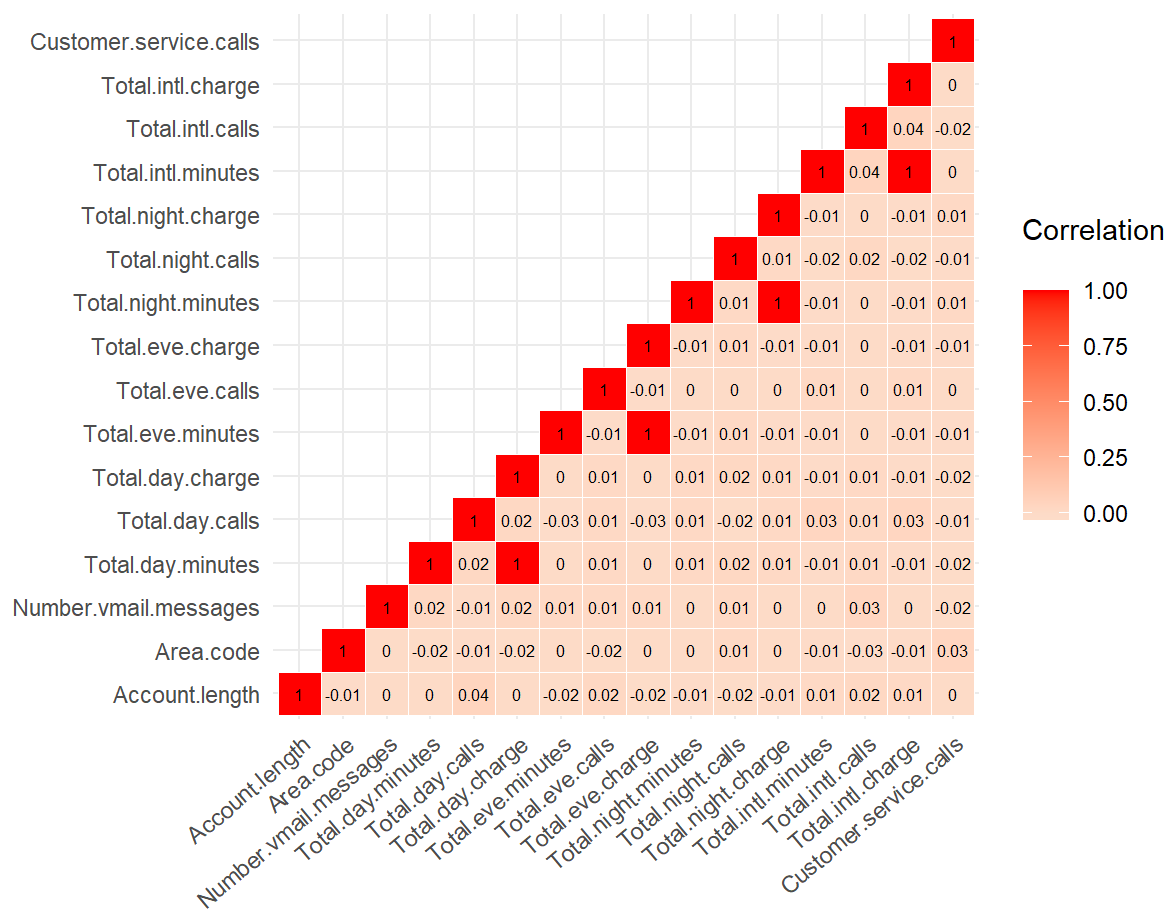
\includegraphics[scale=1]{images/corr.png}
	\end{figure}
	
	As we can see above, the vast majority of the features are uncorrelated. But the pairs like total minutes/total charge are perfectly correlated, which makes sense if users are charged by minutes used. We choose to remove the charge variables to avoid multicollinearity.
	
	Visualizing the distribution of some variables we can find interesting patterns. In Figure \ref{voicemail} we see that among churners, we have fewer customers with voice mail plan (approximately 16.75\%) comparing with non-churners subscribed to this plan (approximately 29.32\%). On the other hand, we have much more churners with an international plan, comparing with non-churners, as shown in Figure \ref{international}. A possible explanation would be that international plan subscribers are finding better offers in this service with competitors.
	
	\begin{figure}[!htb]
		\begin{subfigure}{.5\textwidth}
		\centering
		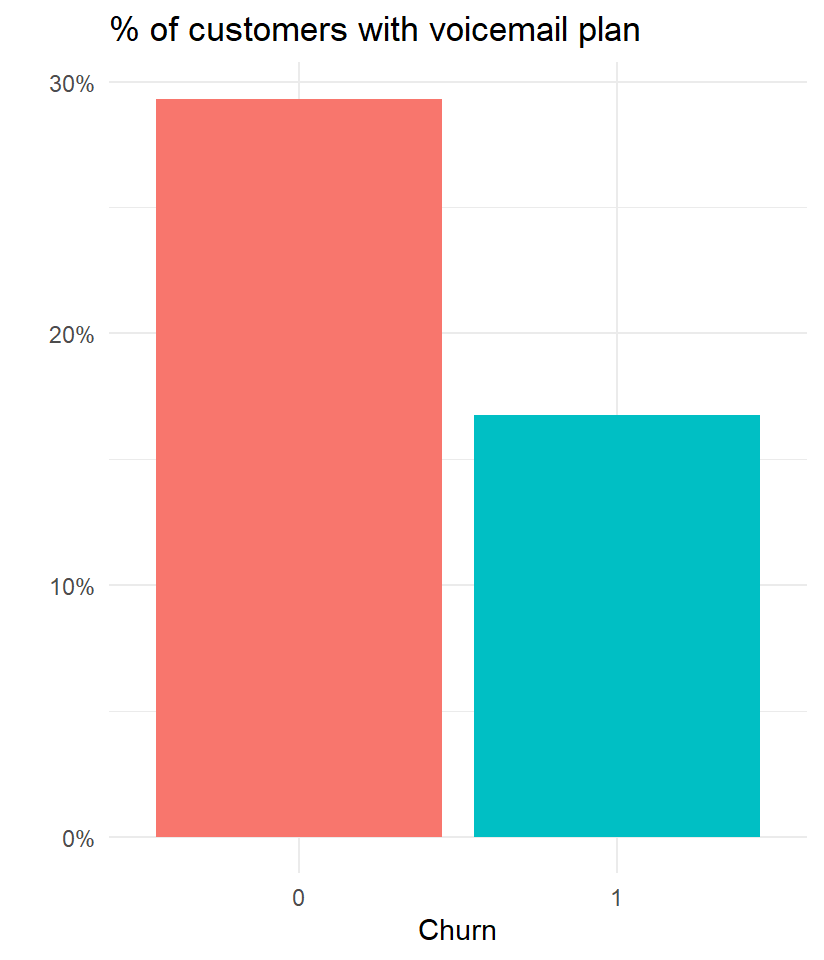
\includegraphics[scale=0.7]{images/voicemail.png}
		\caption{Voicemail clients proportion}
		\label{voicemail}
	\end{subfigure}
	\begin{subfigure}{.5\textwidth}
		\centering
		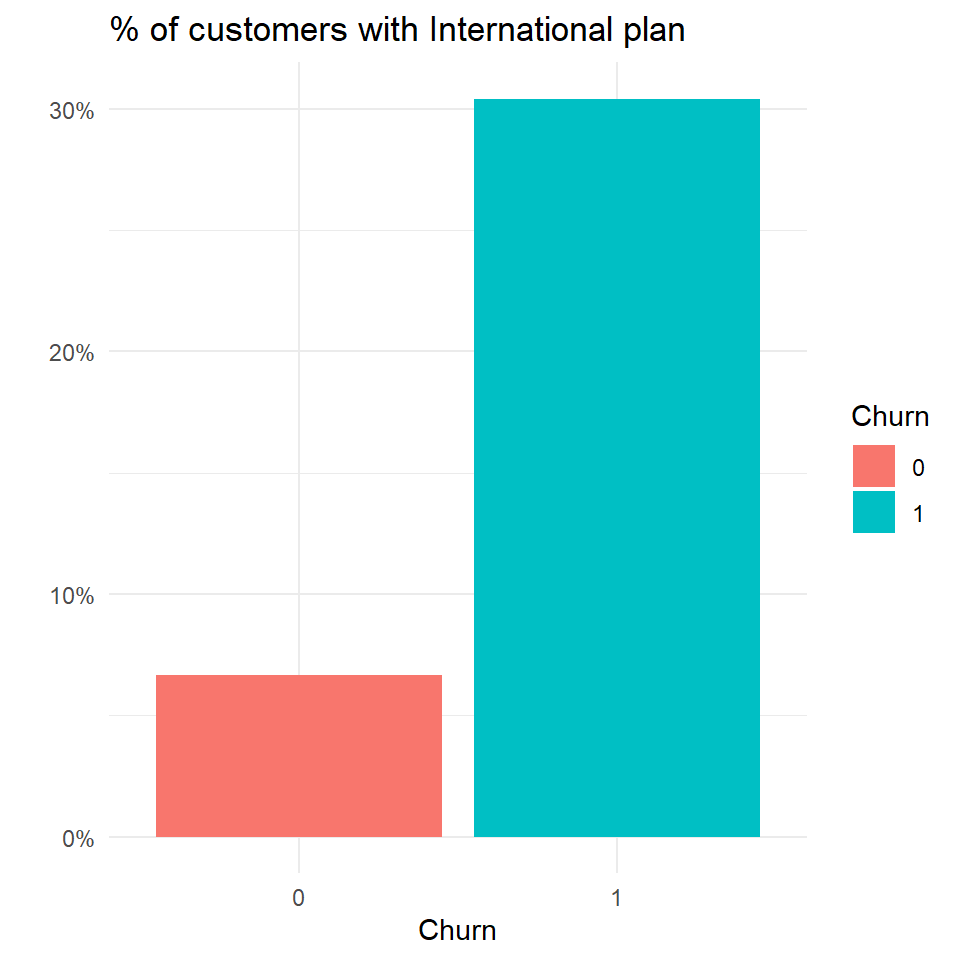
\includegraphics[scale=0.7]{images/international.png}
		\caption{International plan clients proportion}
		\label{international}
		\end{subfigure}
	\caption{Categorical Variables}
	\end{figure}

	Another insightful plot is the one in Figure \ref{cus_services}. We can see that churners make more calls to customer services than non-churners; these calls may be related to complaints about the services and unsatisfactory manifestations.
	
	\begin{figure}[!htb]
		\centering
		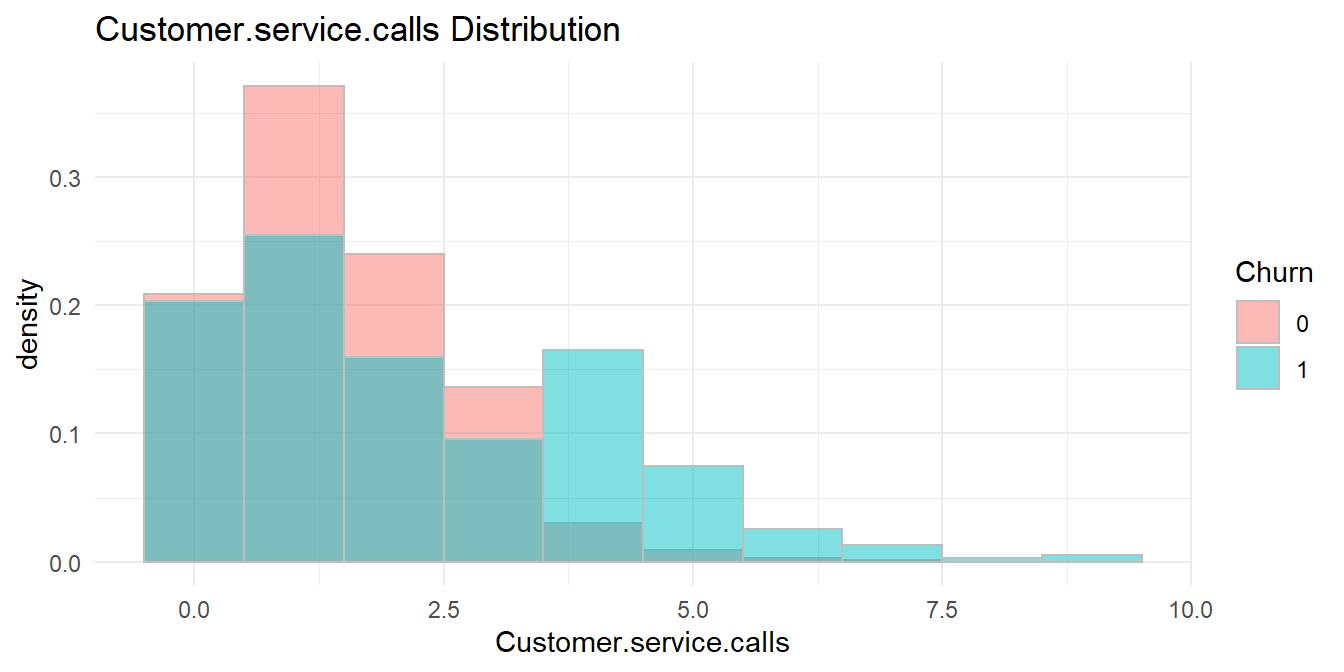
\includegraphics[scale=0.685]{images/customer_services.png}
		\caption{Customer services calls distribution}
		\label{cus_services}
	\end{figure}

Taking a look at the regional distribution in Figure \ref{region}, although Northeast and South regions have more churners, the churn percentage in all of them is around 14.6\% which is the percentage in the training set as a whole.
	\begin{figure}[!htb]
		\centering
		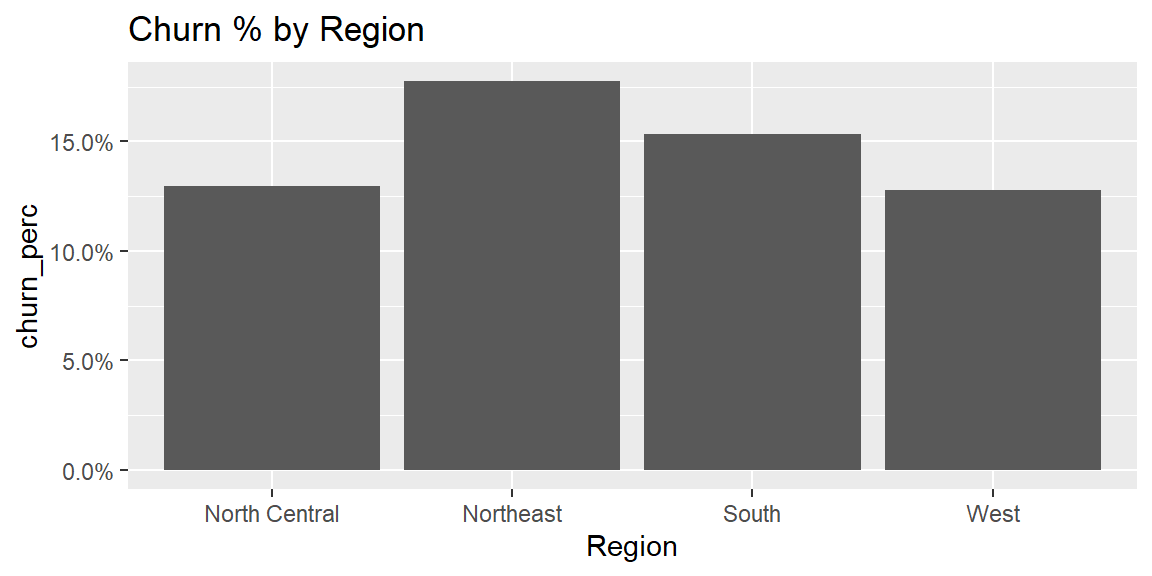
\includegraphics[scale=0.685]{images/region.png}
		\caption{Churners distribution by region}
		\label{region}
	\end{figure}

About the percentage of churners, an approximate proportion of 14\% in the training and test set (see Figure \ref{imbalance}) might be a problem for classifier algorithms because the sample will bias the learning models to the majority class (non-churners). These models may behave poorly in the prediction power of the minority class (churners). In the next section, we discuss some ways to handle this potential problem.

\begin{figure}[!htb]
	\centering
	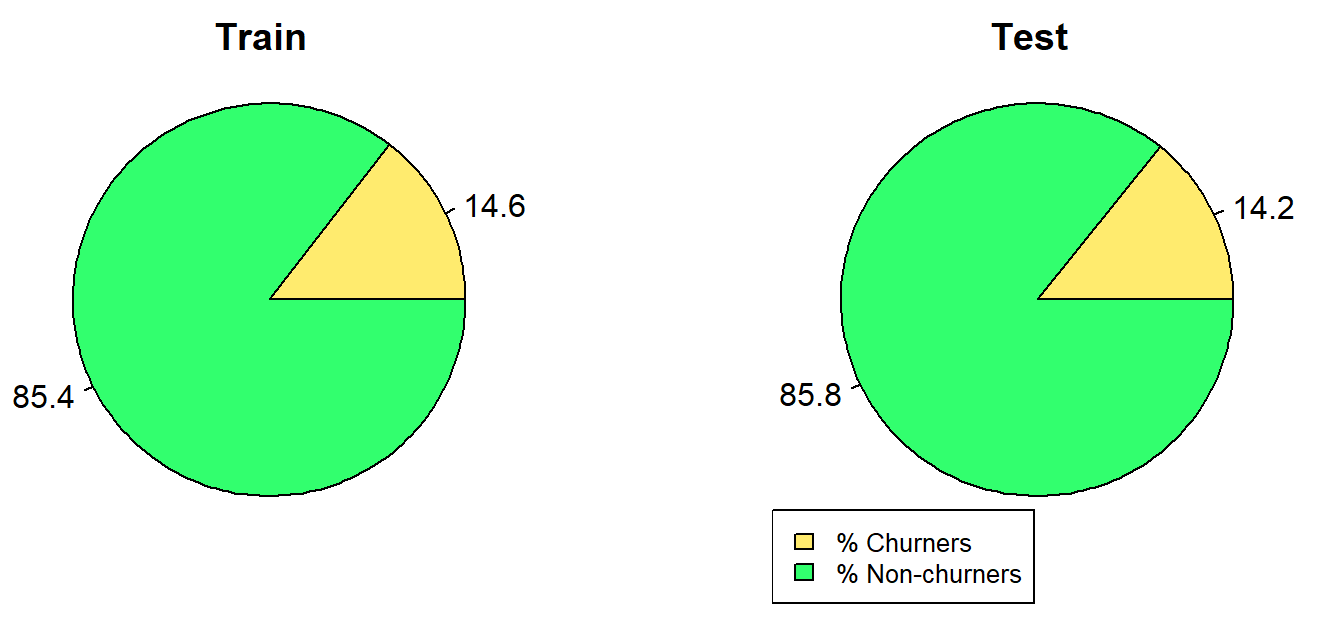
\includegraphics[scale=0.7]{images/imbalance.png}
	\caption{Churners percentage by dataset}
	\label{imbalance}
\end{figure}
	\newpage
	\section{Classification Methods}
	\subsection{Evaluation Metrics}
	The task of churn prediction is a binary classification problem, i.e we have a $n\times p$ features matrix $\bd X$, and a target column vector $\bd y \in \{0,1\}^{n}$, which represents churners as stated in the introduction. We want to learn functions  that receive an $p$-dimensional feature input and outputs a binary value, 0 or 1.
	
	With a learned function/model in hands we can apply it in our test set and build the Confusion Matrix which summarizes how the model has performed.
	
	%https://tex.stackexchange.com/questions/20267/how-to-construct-a-confusion-matrix-in-latex
	\renewcommand\arraystretch{1.5}
\setlength\tabcolsep{0pt}
\begin{table}[!htb]
	\centering
	\begin{tabular}{c >{\bfseries}r @{\hspace{0.7em}}c @{\hspace{0.4em}}c @{\hspace{0.7em}}l}
		\multirow{10}{*}{\parbox{1.1cm}{\bfseries\raggedleft Actual\\ Value}} & 
		& \multicolumn{2}{c}{\bfseries Model Outcome} & \\
		& & \bfseries 1 & \bfseries 0 \\
		& 1 & \MyBox{(TP) True}{Positive} & \MyBox{(FN) False}{Negative}  \\[2.4em]
		& 0 & \MyBox{(FP) False}{Positive} & \MyBox{(TN) True}{Negative}  \\
	\end{tabular}
\caption{Confusion Matrix}
\end{table}

From this table we can derive the following metrics:
\begin{itemize}
	\item Accuracy: (TP+TN)/N;
	\item Recall: TP/(TP+FN),
\end{itemize}
where N is the total number of test observations (TP+TN+FP+FN). Accuracy measures what proportion of the test set our model predicted correctly. When dealing with class imbalance, a model which assigns the majority class to everyone will have high accuracy but will perform poorly in predicting positive instances (churners).

The goal of our prediction algorithm is to correctly identify churners to proactively prevent customer loss. So, in this case, a False Negative has much more impact than a False positive, because the company wants to predict as many churners as possible before they churn. A False Negative may lead to a customer loss that would be avoidable if predicted correctly, but targeting an offer/discount to a False Positive that wouldn't churn is not too harmful, because this client will stay loyal to the company.

Recall aims to measure prediction power among positive instances, i.e the proportion of actual churners we're capturing by the algorithm.

We're also gonna use the \textbf{AUC-ROC} metric, a number between 0 and 1 with measures the area under ROC curve, which is generated plotting false positive rate (FP/(FP+TN)) against true positive rate (TP/(TP+FN)) using different probability/odds thresholds outputted from models. A random classifier will have an AUC equal to $0.5$.

Another important metric, widely used in literature and industry is the \textbf{lift}\cite{class_imbalance}. If the model yields probabilities, we sort the test predictions by these probabilities in a descending order, then we define the lift as the ratio between the percentage of positive entries in the top 10\% lines ($\beta_ {10\%}$), and the percentage of churners (positives) in the entire test set ($\beta_0$). We then define the \textbf{top-decile-lift} as the fraction:
$$\dfrac{\beta_{10\%}}{\beta_0}$$

We can use other percentile values instead of 10\%, but we'll use the decile version since it's widely used performance metric for this kind of problem. A top-decile lift of 2 means that the model classifies two times more churners in the top 10\% group than a random classifier. We’ll devote special attention to recall and top-decile lift and recall because of the imbalance problem. If a model predicts 0 to every test observation, it would be approximately 85\% accurate, but recall would be zero, and lift undefined.



	\subsection{models}
	.... breafly describe ML methods (Knn, logistic regression, naive bayes (maybe) bagging, random forest, boosting, SVM) 
	
	\subsection{Resampling methods}
	The reference\cite{class_imbalance} presents a lot of data-level solutions to deal with class imbalance. The goal is to resample our training set to create a rebalanced new one. We'll focus on the three techniques mentioned below:
	
	\begin{itemize}
		\item (ROS) Random Oversampling: randomly replicates churners instances;
		\item (RUS) Random Undersampling: randomly eliminates the non-churners instances;
		\item (SMOTE) Synthetic minority oversampling technique\cite{smote}
	\end{itemize}
	
	With undersampling, we might be removing valuable information from the dataset. Oversampling may cause biased observations since we're going to replicate observations several times to rebalance the data. 
	
	Smote oversamples the minority class in a smarter way, creating synthetic new data. To do that, for each existing (churner) observation SMOTE selects a random point out of the k-nearest-neighbors (we'll use the default k=5) and creates a new point by performing a random linear interpolation between the point in consideration and the selected neighbor. The article \cite{smote} shows details of this algorithm. We'll use the R implementation of performanceEstimation package\cite{performanceestimation}
	
	\section{Results}
	present and discuss metric's table ...
	
	\section{Conclusions and Future Work}
	\newpage
	\addcontentsline{toc}{section}{References}
	%			\bibliography{refs}
	\printbibliography
\end{document}